\documentclass[12pt]{article}
\usepackage[utf8]{inputenc}
\usepackage[margin=1in]{geometry}
\usepackage[spanish]{babel}\decimalpoint
\usepackage{setspace}\onehalfspacing
\usepackage{parskip} % Espacio entre parrafos.
\usepackage{graphicx} % Para usar comando \includegraphics[]{}
\usepackage{amssymb} % Para usar el simbolo del conj. de los Reales.
\usepackage{amsmath} % Para usar columnas vectoriales.
\usepackage{multirow} % Para unir multiples filas en una tabla.
\usepackage{hyperref} % Siempre debe ser el ultimo paquete.


\setcounter{tocdepth}{2} % Que no incluya subsubsections en la tabla de contenidos (toc).

%================================

\title{Clase 24. Integración Numérica.}
\author{MIT 18.01: Single Variable Calculus.}
\date{}


\begin{document}

\maketitle

\begin{abstract}
\noindent Continuaremos aplicando las integrales para calcular la probabilidad de un evento. Luego, nos centraremos en un conjunto de métodos agrupados en lo que se conoce como integración numérica y que nos permiten calcular de forma numérica (ya no solo analítica, con los TFC) una integral definida.
\end{abstract}


\section{Probabilidades (Continuación).}

Recordemos\footnote{Más detalles, revisar los apuntes de la Clase 23.} que cuando tenemos infinitos valores, podemos calcular la probabilidad de elegir aleatoriamente un punto en $x$  que esté adentro del intervalo $a \leq x_{1} < x_{2} \leq b$ como:
\[
  P(x_{1} < x < x_{2}) = \frac{\int_{x_{1}}^{x_{2}} w(x)dx}{\int_{a}^{b} w(x)dx}
\]
Teniendo esta fórmula en mente, veamos el siguiente ejemplo.

\textbf{Ejemplo 1.} Suponga que una niña está tirando dardos a un tablero y, de un momento a otro, su hermano menor se ubica al lado de éste.

\begin{figure}[hbt!]
\centering
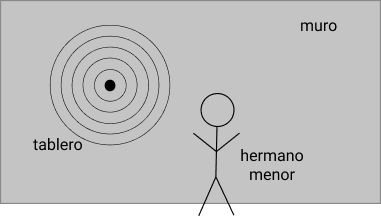
\includegraphics[scale=0.6]{img/darts-prob-example-1.jpg}
\end{figure}

\newpage

Calcule la probabilidad de que uno de los dardos lanzado por la niña golpee a su hermano, asumiendo que:

1) El número de tiros acertados al tablero, $N$, por la niña para cada unidad de radio $r$, es proporcional a $\exp(-r^{2})$.
\[
  N = c \cdot \exp(-r^{2}) \qquad (c = \text{constante de proporcionalidad})
\]
2) La probabilidad de que la niña alcance el blanco del tablero, de radio $r = a$, es de $1/2$.

3) El hermano menor es modelado como la parte de una sección del tablero, encontrándose a una distancia de dos veces el radio del blanco, cubriendo una longitud que va desde las 3 en punto a las 5 en punto en dirección a favor de las manecillas de un reloj.

\begin{figure}[hbt!]
\centering
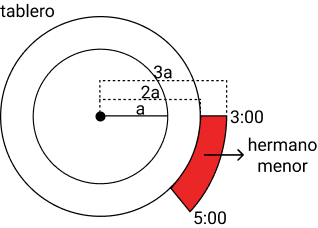
\includegraphics[scale=0.6]{img/darts-prob-example-2.jpg}
\end{figure}

\textbf{Solución.} El problema que estamos tratando es uno de probabilidad. Por lo tanto, vamos a configurarlo de la siguiente manera:
\[
  P(\text{Dardo golpee a su hermano menor}) = \frac{\text{N}^{\underline{\circ}} \text{ dardos que alcanzan a su hermano}}{\text{N}^{\underline{\circ}} \text{ dardos llegando a todos lados}}
                                            = \frac{\text{Parte}}{\text{Todo}}
\]
Puesto que estamos modelando la ubicación del hermano menor como la parte de una sección circular, comencemos calculando aquella superficie como un anillo, dividiendo el tablero de los dardos en dos círculos concéntricos\footnote{Es decir, comparten el mismo centro.}, donde el interno es de radio $r = r_{1}$ y el externo de $r = r_{2}$, con $r_{1} > r_{2}$.

\newpage

\begin{figure}[hbt!]
\centering
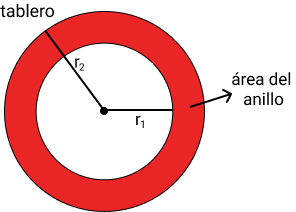
\includegraphics[scale=0.6]{img/darts-prob-example-3.jpg}
\end{figure}

Para calcular el área del anillo, usaremos la función de los lanzamientos de dardos acertados al tablero por parte de la niña, $N = c \cdot \exp(-r^{2})$, cuya gráfica sigue una distribución normal porque la mayoría de ellos caen cercanos a $r = 0$, que es donde está el blanco.

\begin{figure}[hbt!]
\centering
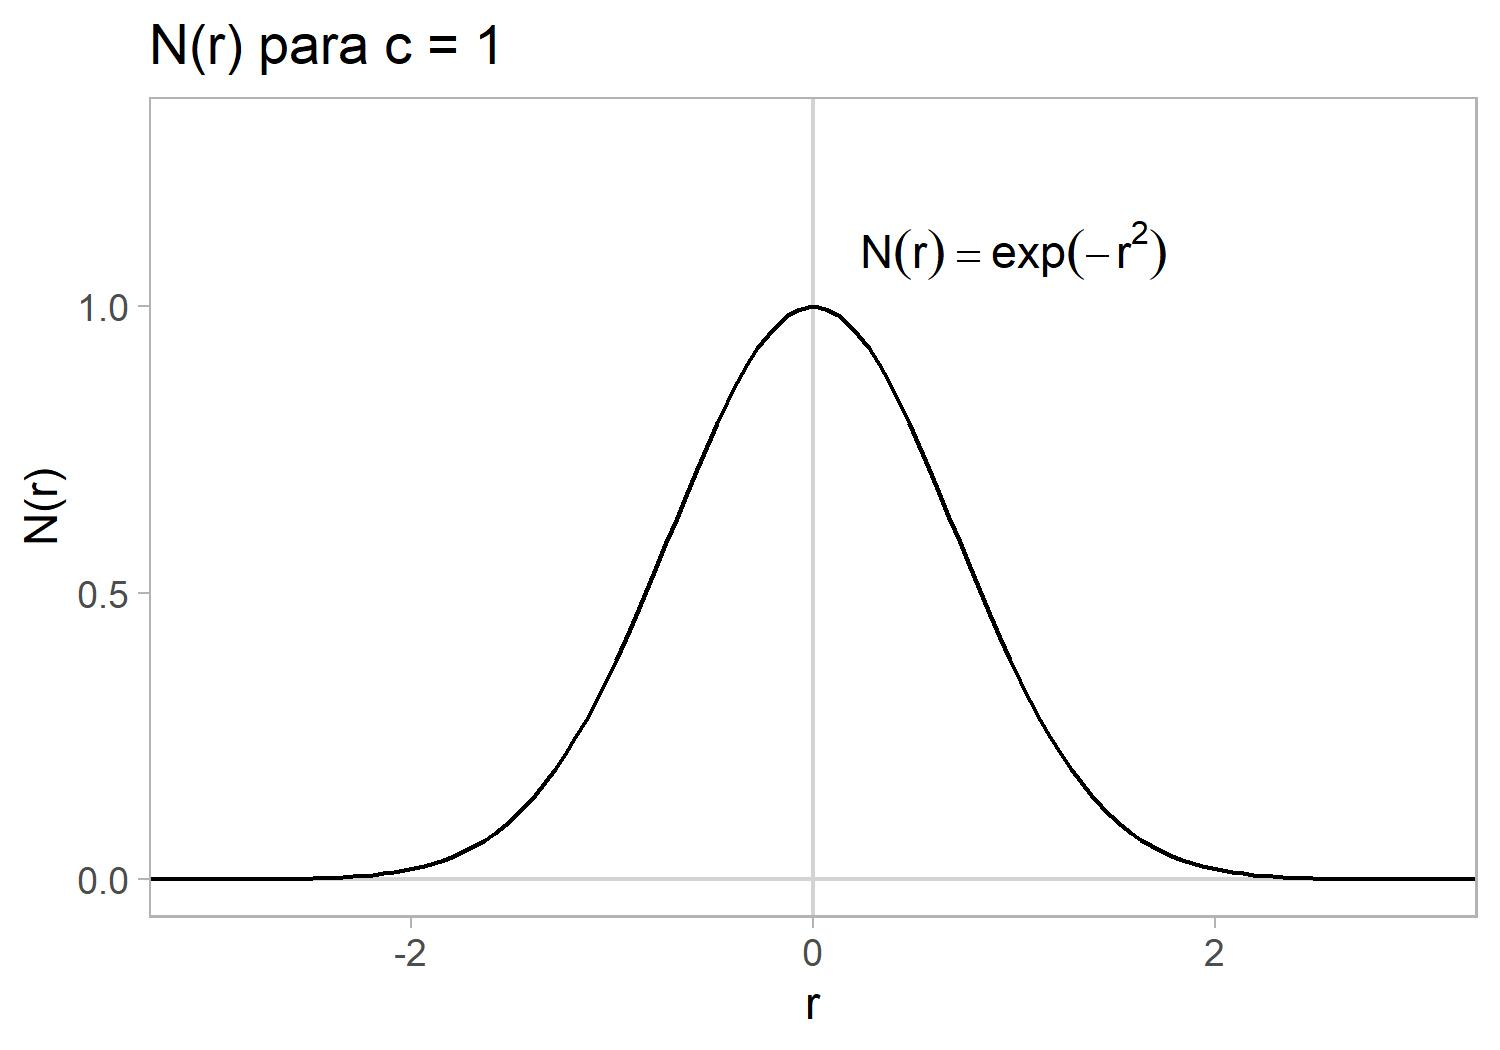
\includegraphics[scale=0.8]{img/darts-prob-example-4.jpg}
\end{figure}

Recordemos que $N(r)$ es la cantidad de tiros que alcanzan el tablero por unidad de radio. Si calculamos el área bajo su curva y sobre $y = 0$ en $[r_{1}, \ r_{2}]$, obtendremos la longitud de $r$ y no del área el anillo en dicho intervalo. Por consiguiente, lo correcto es calcular el \textbf{sólido de revolución} de esta función para abarcar esa superficie, usando el \textbf{método del caparazón cilíndrico}\footnote{Revisar Clase 22.}.

\newpage

\begin{figure}[hbt!]
\centering
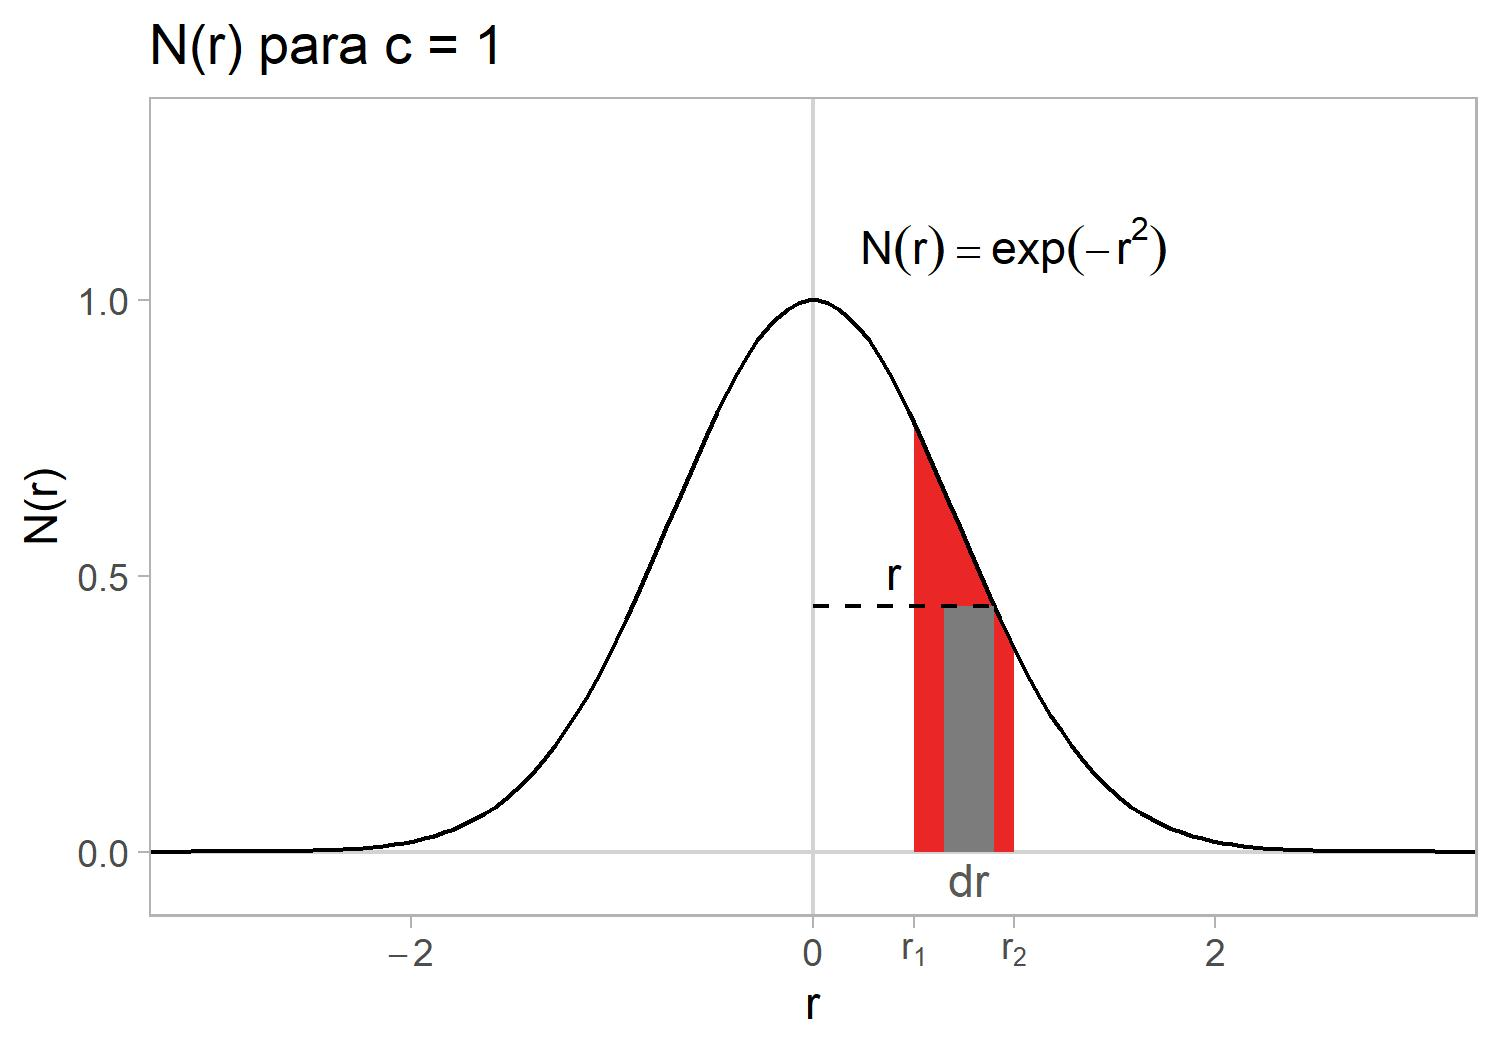
\includegraphics[scale=0.8]{img/darts-prob-example-5.jpg}
\end{figure}

Para aplicar el volumen del caparazón cilíndrico, multiplicamos el perímetro de una sección transversal de radio $r$, por su altura $c \cdot \exp(-r^{2})$ y por el ancho del caparazón, $dr$. En cuanto a la integral (i.e, la suma de todos los volúmenes), la calcularemos entre $r_{1} < r < r_{2}$. Por lo tanto, el área del anillo $A_{an}$ corresponde a:
\[
  A_{an} = \int_{r_{1}}^{r_{2}} [(2 \pi r) \cdot (c \cdot \exp(-r^{2}))] dr
         = 2 \pi c \cdot \left[\int_{r_{1}}^{r_{2}}[r \cdot \exp(-r^{2})] dr \right]
\]
Podemos calcular la integral usando el método de sustitución\footnote{Revisar Clase 19.}, estableciendo que $u = -r^{2}$, de manera que $du = -2rdr$, mientras que sus límites inferior y superior serán $u_{1} = -r_{1}^{2}$ y $u_{2} = -r_{2}^{2}$, respectivamente.
\begin{align*}
  A_{an} &= 2 \pi c \cdot \left[\int_{-r_{1}^{2}}^{-r_{2}^{2}}\left(-\frac{1}{2} \cdot \exp(u)\right) du \right] \\
         &= -\frac{1}{2} \cdot 2 \pi c \cdot [\exp(u)]_{-r_{1}^{2}}^{-r_{2}^{2}} \\
         &= -\pi c \cdot [\exp(-r_{2}^{2}) - \exp(-r_{1}^{2})] \\
  A_{an} &= \pi c \cdot [\exp(-r_{1}^{2}) - \exp(-r_{2}^{2})]
\end{align*}
Teniendo el área del anillo, calculemos la probabilidad de que el dardo lanzado por la niña caiga en éste, $P(r_{1} < r < r_{2})$. La ``Parte'' o la cantidad de veces que los dardos caen en aquella superficie, es $A_{an}$, mientras que el ``Todo'' será el número de dardos que terminan en todos lados, incluyendo el blanco del tablero.

La cantidad de dardos tirados por la niña y que alcanzan el tablero, están dados por $N(r) = c \cdot \exp(-r^{2})$. Por lo tanto, es posible volver a usar la integral de $A_{an}$ para obtener el ``Todo'', pero evaluada en $0 \leq r < \infty$, ya que $r = 0$ se refiere al blanco del tablero, mientras que $r = \infty$ es una buena manera de expresar que el dardo golpea en cualquier otro lugar. Lo anterior implica que debe cumplirse la igualdad $P(0 \leq r < \infty) = 1$.

Entonces, el área del ``Todo'' $A_{T}$ lo calculamos como:
\[
  A_{T} = \pi c \cdot [\exp(-0^{2}) - \exp(-\infty^{2})] = \pi c \cdot (1 - 0) = \pi c
\]
Así, la probabilidad de que un dardo lanzado por la niña caiga en el área del anillo, es:
\[
  P(r_{1} < r < r_{2}) = \frac{A_{an}}{A_{T}}
                       = \frac{\pi c \cdot [\exp(-r_{1}^{2}) - \exp(-r_{2}^{2})]}{\pi c}
                       = \exp(-r_{1}^{2}) - \exp(-r_{2}^{2})
\]
Ahora vayamos a calcular la probabilidad de que el dardo golpee al hermano menor de la niña.

Uno de los supuestos que se señaló en el problema, es que la probabilidad de que la niña alcance el blanco del tablero al lanzar un dardo, es de $1/2$, donde $r = a$ es el radio de este punto:
\[
  P(0 \leq r < a) = \frac{1}{2}
\]
Sabemos que $P(r_{1} < r < r_{2}) = \exp(-r_{1}^{2}) - \exp(-r_{2}^{2})$. Si reemplazamos los valores de esta probabilidad con la que vemos en la ecuación de arriba, obtendremos que:
\begin{align*}
  P(0 \leq r < a) &= \frac{1}{2} \\
  \exp(-0^{2}) - \exp(-a^{2}) &= \frac{1}{2} \\
  1 - \exp(-a^{2}) &= \frac{1}{2} \\
  \exp(-a^{2}) &= \frac{1}{2}
\end{align*}
Por otra parte, el hermano menor está a dos veces el radio del blanco, o entre $2a < r < 3a$, y cubre un área que va desde las 3 en punto a las 5 en punto en dirección favorable a las manillas de un reloj. Es decir, si dividimos el anillo en 12 partes (como un reloj), el lugar donde se encuentra él serían dos partes de esta superficie:
\[
  \text{lugar hermano menor} = \frac{2}{12} = \frac{1}{6}
\]
En consecuencia, la probabilidad de que la niña golpee a su hermano menor con un dardo al lanzarlo al tablero será un sexto del área del anillo entre $2a < r < 3a$:
\begin{align*}
  \frac{1}{6} \cdot P(2a < r < 3a) &= \frac{1}{6} \cdot [\exp(-r_{1}^{2}) - \exp(-r_{2}^{2})] \\
                                   &= \frac{1}{6} \cdot [\exp(-(2a)^{2}) - \exp(-(3a)^{2})] \\
                                   &= \frac{1}{6} \cdot [\exp(-4a^{2}) - \exp(-9a^{2})] \\
  \frac{1}{6} \cdot P(2a < r < 3a) &= \frac{1}{6} \cdot [(\exp(-a^{2}))^{4} - (\exp(-a^{2}))^{9}] \\
\end{align*}
Anteriormente vimos que $\exp(-a^{2}) = 1/2$. Por lo tanto:
\begin{align*}
  \frac{1}{6} \cdot P(2a < r < 3a) &= \frac{1}{6} \cdot \left[\left(\frac{1}{2}\right)^{4} - \left(\frac{1}{2}\right)^{9}\right] \\
                                   &= \frac{1}{6} \cdot \left[\frac{1}{16} - \frac{1}{512}\right] \\
  \frac{1}{6} \cdot P(2a < r < 3a) &\approx 0.01
\end{align*}
La probabilidad de que uno de todos los dardos lanzados al tablero por la niña alcance a su hermano menor, es de casi $1\%$.

Si nos damos cuenta, en este ejemplo la función de ponderación $w(\cdot)$, fue el integrando que obtuvimos del método del caparazón cilíndrico:
\[
  w(r) = (2 \pi r) \cdot (c \cdot \exp(-r^{2}))
\]
Como vemos, es $N(r)$ multiplicado por un factor $2 \pi r$, que es el perímetro del anillo.

La función $w(r)$ es más realista en cuanto al lanzamiento de un dardo al tablero, porque nos muestra que la posibilidad de alcanzar el blanco se reduce mientras nos acercamos a este o, en otras palabras, a medida que $r \to 0$, como podemos verlo en su gráfica:

\newpage

\begin{figure}[hbt!]
\centering
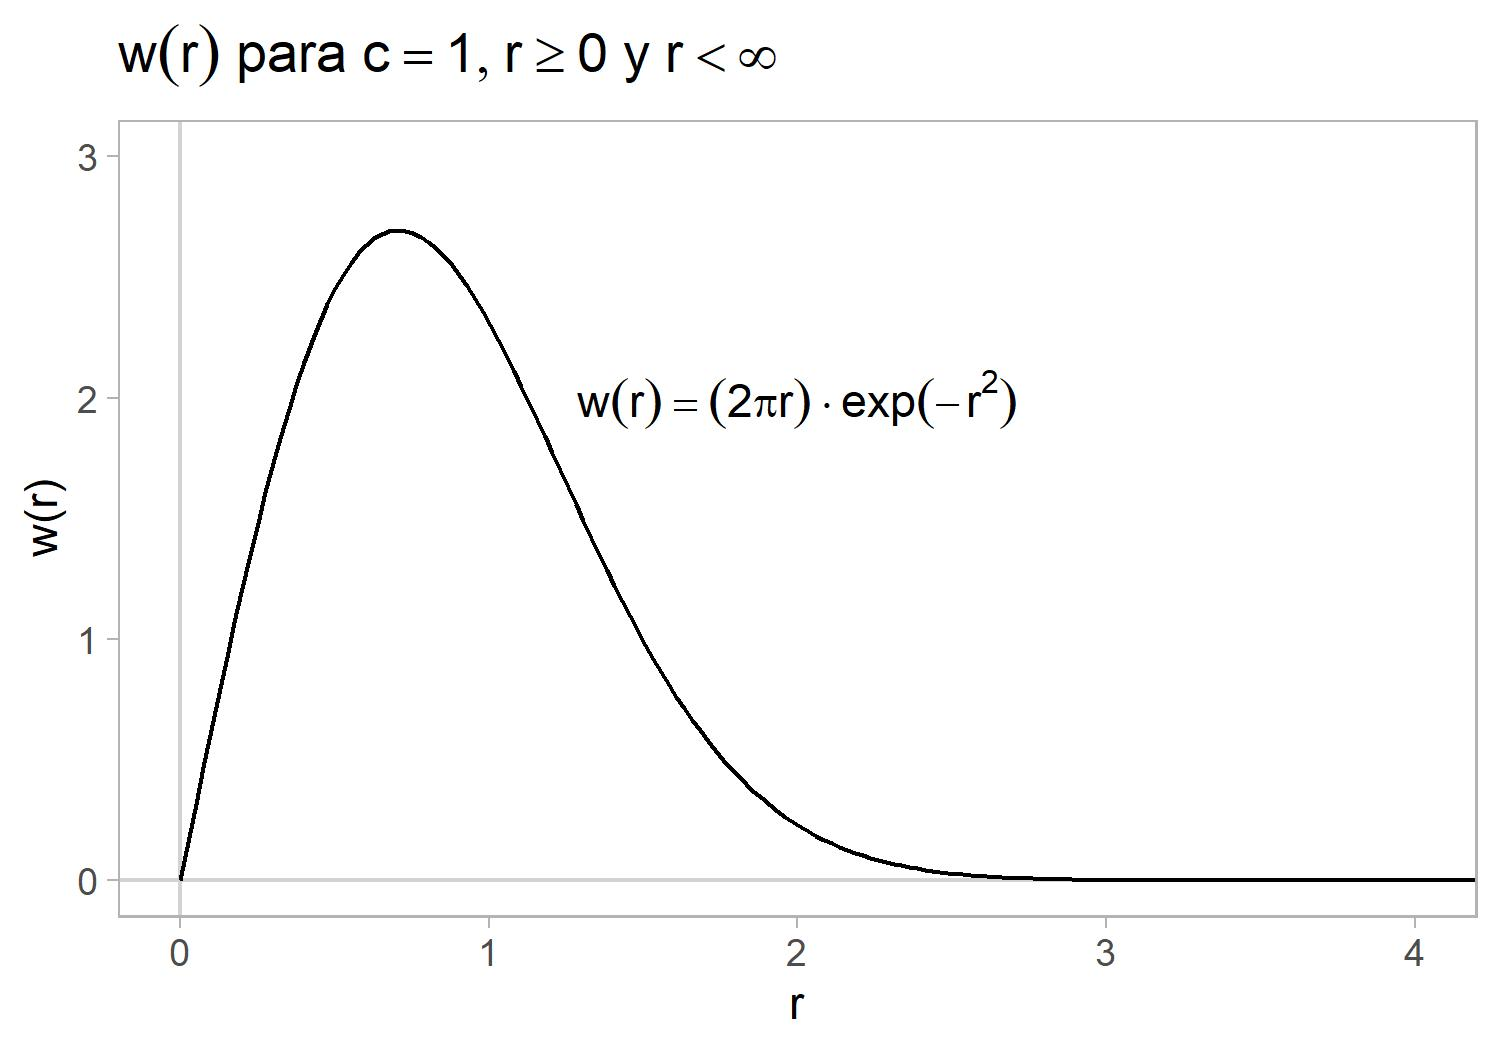
\includegraphics[scale=0.8]{img/darts-prob-example-6.jpg}
\end{figure}


\section{Integración Numérica.}

Hasta ahora sabemos calcular una integral definida de forma analítica, buscando su antiderivada y evaluándola en sus límites. Sin embargo, no siempre es sencillo o, incluso, posible resolverlas de esa forma. En esos casos, podemos \textbf{aproximarnos a su valor} usando alguno de los distintos métodos que, en conjunto, reciben el nombre de \textbf{Integración Numérica}.

En esta ocasión, estudiaremos tres métodos de integración numérica: La suma de Riemann (método del rectángulo), la regla del trapezoide y la regla de Simpson.

\subsection{Suma de Riemann o Método del Rectángulo.}

Un método de aproximación numérica a una integral definida es el \textbf{del Rectángulo}, que también corresponde a la \textbf{suma de Riemann}.

Como ya hemos estudiado, la suma de Riemann consiste en dividir muchas veces de forma vertical un área bajo/sobre una curva que va entre $a \leq x \leq b$:
\[
  a = x_{0} < x_{1} < x_{2} < \cdots < x_{n} = b
\]
Con cada división formamos \textbf{rectángulos} de largo $\Delta x = x_{i} - x_{i - 1}$, para $i = 1, \ 2, \ \cdots, \ n$. La altura de estas figuras la obtenemos \textbf{evaluando la función} para cada $x_{i}$.
\[
  y_{0} = f(x_{0}), \ y_{1} = f(x_{1}), \ \cdots, y_{n} = f(x_{n})
\]
Lo anterior implica a nivel geométrico que los rectángulos siempre tocan a la curva de $f(x)$, como lo vemos a continuación:

\begin{figure}[hbt!]
\centering
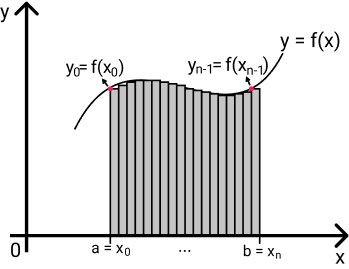
\includegraphics[scale=0.6]{img/riemann-sum-num-int.jpg}
\end{figure}

La suma de Riemann consiste en sumar las alturas de los rectángulos y multiplicarlas por sus anchos $\Delta x$. Si comenzamos con el punto $(x_{0}, \ y_{0})$, pasa a llamarse \textbf{suma izquierda de Riemann}, mientras que con $(x_{1}, \ y_{1})$ recibe el nombre de \textbf{suma derecha de Riemann}.
\begin{align*}
  &\text{Suma izquierda} \rightarrow \int_{a}^{b} f(x)dx \approx (y_{0} + y_{1} + \cdots + y_{n - 1}) \cdot \Delta x \\
  &\text{Suma derecha} \rightarrow \int_{a}^{b} f(x)dx \approx (y_{1} + y_{2} + \cdots + y_{n}) \cdot \Delta x
\end{align*}
También existen las sumas inferior y superior de Riemann, las cuales son iguales a las dos anteriores dependiendo si la función $f(x)$ del integrando es creciente o decreciente. Esto lo resumimos en la siguiente tabla:

\begin{table}[hbt!]
\centering

\begin{tabular}{c c c}
\hline
& \multicolumn{2}{c}{Función} \\
\cline{2-3}
Riemann & Creciente & Decreciente \\
\hline
Izquierda & Inferior & Superior \\
Derecha & Superior & Inferior \\
\hline
\end{tabular}

\end{table}

\subsection{Regla del Trapezoide.}

Un segundo método de aproximación numérica a una integral definida, es la \textbf{Regla del Trapezoide}. Acá también dividimos el área bajo/sobre la curva de la función de forma vertical, pero unimos los puntos superiores con \textbf{rectas diagonales}, formando \textbf{trapezoides} en vez de rectángulos.

\newpage

\begin{figure}[hbt!]
\centering
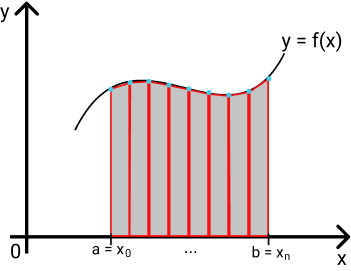
\includegraphics[scale=0.6]{img/trapezoidal-rule-num-int.jpg}
\end{figure}

Veamos el trapezoide que se forma entre $x_{3}$ y $x_{4}$ de manera horizontal.

\begin{figure}[hbt!]
\centering
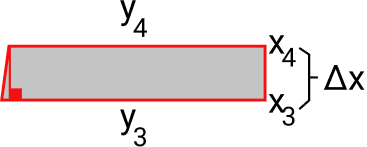
\includegraphics[scale=0.6]{img/trapezoidal-rule-num-int-2.jpg}
\end{figure}

Como se puede apreciar, en términos estrictos las bases del trapezoide son $y_{3}$ e $y_{4}$, mientras que su altura está dada por $\Delta x = x_{4} - x_{3}$. El área de esta figura, $A_{Tr}$,  se calcula como el producto entre su altura y el promedio de sus bases:
\[
  A_{Tr} = \Delta x \cdot \left(\frac{y_{3} + y_{4}}{2}\right)
\]
Por lo tanto, la \textbf{fórmula de la regla del trapezoide} es igual al producto entre las alturas (que son iguales) $\Delta x$ y la suma de los promedios de sus bases:
\begin{align*}
  \int_{a}^{b} f(x)dx &\approx \Delta x \cdot \left(
      \frac{y_{0} + y_{1}}{2} + \frac{y_{1} + y_{2}}{2} + \frac{y_{2} + y_{3}}{2} + \cdots + \frac{y_{n - 1} + y_{n}}{2}
    \right) \\
                      &= \Delta x \cdot \left(\frac{y_{0}}{2} + y_{1} + y_{2} + y_{3} + \cdots + y_{n - 1} + \frac{y_{n}}{2}\right)
\end{align*}
La fórmula de la regla del trapezoide coincide con ser igual al \textbf{promedio de las sumas de la izquierda y derecha de Riemann}.
\begin{align*}
\int_{a}^{b} f(x)dx &\approx \Delta x \cdot \left(\frac{y_{0}}{2} + y_{1} + y_{2} + y_{3} + \cdots + y_{n - 1} + \frac{y_{n}}{2}\right) \\
                    &= \Delta x \cdot \left[\frac{(y_{0} + y_{1} + \cdots + y_{n - 1}) + (y_{1} + y_{2} + \cdots + y_{n})}{2}\right]
\end{align*}

\subsection{Regla de Simpson.}

El tercer método de aproximación que veremos, recibe el nombre de \textbf{Regla de Simpson}. Comenzamos dividiendo el área bajo/sobre la curva de $f(x)$ y sobre/bajo $a \leq x \leq b$ con rectas verticales, pero la \textbf{cantidad de particiones} $n$ debe ser un \textbf{número entero par}. Aquello se debe a que estimaremos el valor de la integral usando \textbf{parábolas}.

En particular, en la regla de Simpson trazamos parábolas que se ajusten mejor a cada par de divisiones y calculamos el área abajo de cada una de ellas. Posteriormente, las sumamos para obtener la aproximación de la superficie de $f(x)$ en $[a, \ b]$.

\begin{figure}[hbt!]
\centering
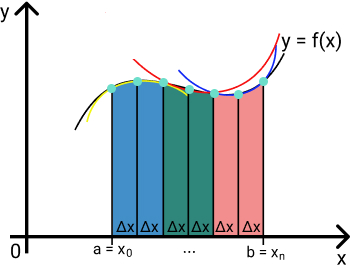
\includegraphics[scale=0.6]{img/simpson's-rule-num-int.jpg}
\end{figure}

El área abajo de una parábola entre dos particiones, que denotaremos como $A_{P}$, se calcula como el producto entre la base de la figura y un promedio ponderado entre las alturas:
\[
  A_{P} = 2\Delta x \cdot \left(\frac{y_{0} + 4y_{1} + y_{2}}{6}\right) = \frac{\Delta x}{3} \cdot (y_{0} + 4y_{1} + y_{2})
\]
El primer paréntesis está dividido por seis porque esa es la cantidad de $y_{i}$s que se están sumando.

En la siguiente demostración veremos cómo se proviene esta fórmula.

\textbf{Demostración.} Considere las funciones $y = f(x)$ y $P(x)$, siendo esta última una parábola y el área abajo de ella entre $[x_{0}, \ x_{2}]$ dividida en dos partes, donde $x_{0} = -h$, $x_{1} = 0$ y $x_{2} = h$.

\newpage

\begin{figure}[hbt!]
\centering
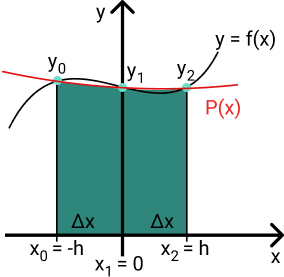
\includegraphics[scale=0.6]{img/simpson's-rule-num-int-2.jpg}
\end{figure}

Comencemos definiendo a $P(x)$ con la ecuación cuadrática general.
\[
  P(x) = Ax^{2} + Bx + C
\]
Luego, calculemos el área abajo $P(x)$ y sobre $-h \leq x \leq h$.
\[
  \int_{-h}^{h} P(x)dx = \left[\frac{Ax^{3}}{3} + \frac{Bx^{2}}{2} + Cx\right]_{-h}^{h} = \frac{2Ah^{3}}{3} + 2Ch
\]
Y factoricemos la integral de arriba por $h/3$.
\[
  \int_{-h}^{h} P(x)dx = \frac{h}{3} \cdot \left(2Ah^{2} + 3(2C)\right) = \frac{h}{3} \cdot \left(2Ah^{2} + 6C\right)
\]
Nuestra próxima tarea, es conocer las constantes $A$ y $C$ de $\int_{-h}^{h} P(x)dx$. En la gráfica de arriba se puede observar que:
\[
  f(x_{0}) = P(x_{0}) = y_{0} \qquad f(x_{1}) = P(x_{1}) = y_{1} \qquad f(x_{2}) = P(x_{2}) = y_{2}
\]
Por lo tanto, el siguiente paso será evaluar $P(x)$ para $x_{0} = -h$, $x_{1} = 0$ y $x_{2} = h$:
\begin{align*}
P(-h) &= Ah^{2} - Bh + C = y_{0} & P(0) &= 0 + 0 + C = y_{1} & P(h) &= Ah^{2} + Bh + C = y_{2}
\end{align*}
Al resolver la siguiente suma de ecuaciones:
\[
\begin{aligned}
\underline{
  \begin{aligned}
  Ah^{2} - Bh + C &= y_{0} \\
  C &= y_{1} \\
  Ah^{2} + Bh + C &= y_{2}
  \end{aligned}
}
\end{aligned}
\]
obtendremos que:
\[
  2Ah^{2} + 3C = y_{0} + y_{1} + y_{2}
\]
Veamos que $C = y_{1}$, la cual podemos reemplazar en la ecuación de arriba:
\[
2Ah^{2} + 3y_{1} = y_{0} + y_{1} + y_{2}
\]
A partir de esta última ecuación podemos conocer a $2Ah^{2}$, despejándola en ella:
\[
  2Ah^{2} = y_{0} - 2y_{1} + y_{2}
\]
Reemplacemos a $C$ y $2Ah^{2}$ en $\int_{-h}^{h} P(x)dx$:
\[
  \int_{-h}^{h} P(x)dx = \frac{h}{3} \cdot (y_{0} - 2y_{1} + y_{2} + 6y_{1}) = \frac{h}{3} \cdot (y_{0} + 4y_{1} + y_{2})
\]
En la gráfica inicial de esta demostración, podemos observar que $h = h - 0 = x_{2} - x_{1} = \Delta x$. En consecuencia, el área abajo de la parábola $P(x)$ entre $-h \leq x \leq h$ es:
\[
  \int_{-h}^{h} P(x)dx = \frac{\Delta x}{3} \cdot (y_{0} + 4y_{1} + y_{2}) = A_{P} \qquad (\text{Q.E.D})
\]
De este modo, la aproximación del área abajo de $f(x)$ en $[a, \ b]$ a partir de la \textbf{regla de Simpson}, será el producto de un tercio de $\Delta x$ y la suma de las superficies abajo de cada parábola.
\begin{align*}
  \int_{a}^{b} f(x)dx &\approx \frac{\Delta x}{3} \cdot
                               ([y_{0} + 4y_{1} + y_{2}] + [y_{2} + 4y_{3} + y_{4}] + \cdots + [y_{n - 2} + 4y_{n - 1} + y_{n}]) \\
                      &= \frac{\Delta x}{3} \cdot (y_{0} + 4y_{1} + 2y_{2} + 4y_{3} + \cdots + 2y_{n - 2} + 4y_{n - 1} + y_{n})
\end{align*}
Los coeficientes del paréntesis siguen un patrón como el que podemos ver en el siguiente Triángulo de Pascal, para tres parábolas:

\begin{table}[hbt!]
\centering

\begin{tabular}{c c c c c c c}
 & & $1$ & $4$ & $1$ & & \\
 & $1$ & $4$ & $2$ & $4$ & $1$ & \\
$1$ & $4$ & $2$ & $4$ & $2$ & $4$ & $1$
\end{tabular}

\end{table}

donde la última fila, que corresponde a los coeficientes que estarán en la aproximación de $\int_{a}^{b} f(x)dx$ para tres parábolas, es posible obtenerla haciendo la siguiente suma:

\newpage

\begin{table}[hbt!]
\centering

\begin{tabular}{c c c c c c c}
$1$ & $4$ & $1$ & & & &  \\
 & & $1$ & $4$ & $1$ & & \\
 & & & & $1$ & $4$ & $1$\\
\hline
$1$ & $4$ & $2$ & $4$ & $2$ & $4$ & $1$
\end{tabular}

\end{table}

Entonces, a modo de síntesis, para calcular de forma numérica una integral definida, tenemos los siguientes tres (de muchos más) métodos de integración numérica:
\begin{align*}
  \text{Riemann} &\rightarrow \int_{a}^{b} f(x)dx \approx \Delta x \cdot (y_{0} + y_{1} + \cdots + y_{n - 1}) \text{ o } \\
                         &\rightarrow \int_{a}^{b} f(x)dx \approx \Delta x \cdot (y_{1} + y_{2} + \cdots + y_{n}) \\
  \text{Trapezoide} &\rightarrow \int_{a}^{b} f(x)dx \approx \Delta x \cdot
                              \left(\frac{y_{0}}{2} + y_{1} + y_{2} + y_{3} + \cdots + y_{n - 1} + \frac{y_{n}}{2}\right) \\
  \text{Simpson} &\rightarrow \int_{a}^{b} f(x)dx \approx
                          \frac{\Delta x}{3} \cdot (y_{0} + 4y_{1} + 2y_{2} + 4y_{3} + \cdots + 2y_{n - 2} + 4y_{n - 1} + y_{n})
\end{align*}
En términos de precisión, podemos ordenarlas como:
\[
  \text{Riemann} < \text{Trapezoide} < \text{Simpson}
\]
aunque ninguna es $100\%$ exacta. Es decir, todas tienen una tasa de error.

\textbf{Ejemplo 2.} Estime $\int_{1}^{2} (1/x)dx$ usando las reglas del trapezoide y de Simpson para dos intervalos (i.e, $n = 2$).

\textbf{Solución.} La integral que buscamos estimar es posible obtenerla de forma analítica, así que comenzaremos calculándola de esa manera.
\[
  \int_{1}^{2} \frac{1}{x} dx = \ln(|x|) |_{1}^{2} = \ln(2) - \ln(1) = \ln(2) - 0 \approx 0.693147
\]
Ahora que tenemos una idea del valor de $\int_{1}^{2} (1/x)dx$, veamos cuánto nos acercamos a partir de los dos métodos de integración numérica de este ejemplo. Algo a tener presente es que la precisión aumenta a medida que $n$ también lo hace, por lo que es esperable que ésta no lo sea tanto para $n = 2$.

Antes de comenzar a trabajar con las dos reglas de integración numérica, primero calculemos $\Delta x$.
\[
  \Delta x = \frac{2 - 1}{2} = \frac{1}{2}
\]
Luego, obtengamos los valores de $y_{0}$, $y_{1}$ e $y_{2}$ con $y = 1/x$, ya que para dividir el área abajo de $y$ en dos necesitamos tres divisiones verticales (los límites superior e inferior más el que va en la mitad).

\begin{table}[hbt!]
\centering

\begin{tabular}{c|c c c}
$x_{i}$ & $1$ & $3/2$ & $2$ \\
\hline
$y_{i}$ & $1$ & $2/3$ & $1/2$
\end{tabular}

\end{table}

Partamos con la regla del trapezoide.
\[
  \int_{1}^{2} \frac{1}{x}dx \approx \frac{1}{2} \cdot \left(\frac{1}{2} + \frac{2}{3} + \frac{1/2}{2}\right) = 0.708\bar{3}
\]
Ahora sigamos con la regla de Simpson.
\[
  \int_{1}^{2} \frac{1}{x}dx \approx \frac{(1/2)}{3} \cdot \left[1 + \left(4 \cdot \frac{2}{3}\right) + \frac{1}{2}\right] = 0.69\bar{4}
\]
Veamos que, a pesar de trabajar con solo dos intervalos, la regla de Simpson sigue siendo bastante precisa.

En general, la \textbf{magnitud de error $\epsilon$ de la regla de Simpson} se puede calcular como:
\[
  \epsilon = \frac{M(b - a)}{180} \cdot (\Delta x)^{4}
           = \frac{M(b - a)}{180} \cdot \left(\frac{b - a}{n}\right)^{4}
           = \frac{M(b - a)^{5}}{180n^{4}}
\]
donde $M$ es el valor máximo del integrando $y_{i} = f(x_{i})$, para $i = 0, \ 1, \ \cdots, \ n$.



\end{document}
